% !iTeXMac(input): POH.tex 
\chapter{LIMITATIONS}
\vspace{\minitocspacebefore}
\minitoc
%\mtcskip
%\minilof
\cleardoublepage
\section{INTRODUCTION}
Section 2 includes operating limitations, instrument markings, and basic placards necessary for the safe operation of
the aircraft, its engine, systems and equipment.

\begin{Note}
  The airspeeds listed in this section are based on the use of the normal static source.  If the alternate static
source is used, the airspeeds should be corrected using the information in Section \ref{perf-sec-number}.
\end{Note}

\section{AIRSPEED LIMITATIONS}
%Altitude TAS CAS
%10000 231.57 200
%12000 231.57 193.95 194
%14000 231.57 187.98 188
%16000 231.57 182.11 182
%18000 231.57 176.32 176
%20000 231.57 170.63 170
%22000 231.57 165.03 164
%24000 231.57 159.52 158
\settowidth\colTwo{\hspace{0.2in}1500 lb (703.1~kg)~or~greater:}
\settowidth\colThree{KIAS}
\settowidth\colFour{KCAS}
\begin{tabularx}{\textwidth}{|c|>{\raggedright}p{\colTwo}|c|c|X|}
\hline
 &SPEED & KIAS & KCAS & REMARKS \\
\hline
\hline
$\mathrm{V_{NE}}$ & Never Exceed Speed & 203 & 200 & Do not exceed this speed in any operation.  Reduce by 3 kt per 1000 ft above 10,000 ft.\\
\hline
$\mathrm{V_{NO}}$  & Maximum Structural\\
Cruising Speed& 170 & 168 & Do not exceed this speed except in smooth air, and then only with
caution.\\
\hline
$\mathrm{V_{A}}$ & Manoeuvring Speed\\
\hspace{0.2in}1550 lb (703.1~kg)~or~greater:\\
\hspace{0.2in}1300 lb (589.7~kg): &\multicolumn{1}{p{\colThree}|}{\centering ~\\
\textcolor{red}{TBD}\\ \textcolor{red}{TBD}} & \multicolumn{1}{p{\colFour}|}{\centering~\\ \textcolor{red}{120}\\
\textcolor{red}{110}}& Do not make full or abrupt control
movements above this speed. \textcolor{red}{These speeds are estimates based on CAFE data. To be updated after flight testing.}\\
\hline
$\mathrm{V_{FE}}$ & Maximum Flap Extended Speed\\
\hspace{0.2in}0\textdegree ~to~20\textdegree ~Flaps:\\
\hspace{0.2in}20\textdegree ~to~40\textdegree ~Flaps:&
\multicolumn{1}{p{\colThree}|}{\centering ~\\ \textcolor{red}{TBD}\\\textcolor{red}{TBD}}&
\multicolumn{1}{p{\colFour}|}{\centering~\\96\\87}
& Do not exceed these speeds with the given flap settings.\\
\hline
\end{tabularx} 

\begin{figure}[h!]
%\includegraphics*[viewport = 0 25 385 265]{../Diagrams/CG_envelope2.ps} % original chart from Grace
  \begin{center}
  % GNUPLOT: LaTeX picture with Postscript
\begingroup
  \makeatletter
  \providecommand\color[2][]{%
    \GenericError{(gnuplot) \space\space\space\@spaces}{%
      Package color not loaded in conjunction with
      terminal option `colourtext'%
    }{See the gnuplot documentation for explanation.%
    }{Either use 'blacktext' in gnuplot or load the package
      color.sty in LaTeX.}%
    \renewcommand\color[2][]{}%
  }%
  \providecommand\includegraphics[2][]{%
    \GenericError{(gnuplot) \space\space\space\@spaces}{%
      Package graphicx or graphics not loaded%
    }{See the gnuplot documentation for explanation.%
    }{The gnuplot epslatex terminal needs graphicx.sty or graphics.sty.}%
    \renewcommand\includegraphics[2][]{}%
  }%
  \providecommand\rotatebox[2]{#2}%
  \@ifundefined{ifGPcolor}{%
    \newif\ifGPcolor
    \GPcolorfalse
  }{}%
  \@ifundefined{ifGPblacktext}{%
    \newif\ifGPblacktext
    \GPblacktexttrue
  }{}%
  % define a \g@addto@macro without @ in the name:
  \let\gplgaddtomacro\g@addto@macro
  % define empty templates for all commands taking text:
  \gdef\gplbacktext{}%
  \gdef\gplfronttext{}%
  \makeatother
  \ifGPblacktext
    % no textcolor at all
    \def\colorrgb#1{}%
    \def\colorgray#1{}%
  \else
    % gray or color?
    \ifGPcolor
      \def\colorrgb#1{\color[rgb]{#1}}%
      \def\colorgray#1{\color[gray]{#1}}%
      \expandafter\def\csname LTw\endcsname{\color{white}}%
      \expandafter\def\csname LTb\endcsname{\color{black}}%
      \expandafter\def\csname LTa\endcsname{\color{black}}%
      \expandafter\def\csname LT0\endcsname{\color[rgb]{1,0,0}}%
      \expandafter\def\csname LT1\endcsname{\color[rgb]{0,1,0}}%
      \expandafter\def\csname LT2\endcsname{\color[rgb]{0,0,1}}%
      \expandafter\def\csname LT3\endcsname{\color[rgb]{1,0,1}}%
      \expandafter\def\csname LT4\endcsname{\color[rgb]{0,1,1}}%
      \expandafter\def\csname LT5\endcsname{\color[rgb]{1,1,0}}%
      \expandafter\def\csname LT6\endcsname{\color[rgb]{0,0,0}}%
      \expandafter\def\csname LT7\endcsname{\color[rgb]{1,0.3,0}}%
      \expandafter\def\csname LT8\endcsname{\color[rgb]{0.5,0.5,0.5}}%
    \else
      % gray
      \def\colorrgb#1{\color{black}}%
      \def\colorgray#1{\color[gray]{#1}}%
      \expandafter\def\csname LTw\endcsname{\color{white}}%
      \expandafter\def\csname LTb\endcsname{\color{black}}%
      \expandafter\def\csname LTa\endcsname{\color{black}}%
      \expandafter\def\csname LT0\endcsname{\color{black}}%
      \expandafter\def\csname LT1\endcsname{\color{black}}%
      \expandafter\def\csname LT2\endcsname{\color{black}}%
      \expandafter\def\csname LT3\endcsname{\color{black}}%
      \expandafter\def\csname LT4\endcsname{\color{black}}%
      \expandafter\def\csname LT5\endcsname{\color{black}}%
      \expandafter\def\csname LT6\endcsname{\color{black}}%
      \expandafter\def\csname LT7\endcsname{\color{black}}%
      \expandafter\def\csname LT8\endcsname{\color{black}}%
    \fi
  \fi
  \setlength{\unitlength}{0.0500bp}%
  \begin{picture}(7200.00,5040.00)%
    \gplgaddtomacro\gplbacktext{%
      \csname LTb\endcsname%
      \put(1342,704){\makebox(0,0)[r]{\strut{}0}}%
      \csname LTb\endcsname%
      \put(1342,1518){\makebox(0,0)[r]{\strut{}5,000}}%
      \csname LTb\endcsname%
      \put(1342,2332){\makebox(0,0)[r]{\strut{}10,000}}%
      \csname LTb\endcsname%
      \put(1342,3147){\makebox(0,0)[r]{\strut{}15,000}}%
      \csname LTb\endcsname%
      \put(1342,3961){\makebox(0,0)[r]{\strut{}20,000}}%
      \csname LTb\endcsname%
      \put(1342,4775){\makebox(0,0)[r]{\strut{}25,000}}%
      \csname LTb\endcsname%
      \put(1474,484){\makebox(0,0){\strut{} 150}}%
      \csname LTb\endcsname%
      \put(2373,484){\makebox(0,0){\strut{} 160}}%
      \csname LTb\endcsname%
      \put(3272,484){\makebox(0,0){\strut{} 170}}%
      \csname LTb\endcsname%
      \put(4172,484){\makebox(0,0){\strut{} 180}}%
      \csname LTb\endcsname%
      \put(5071,484){\makebox(0,0){\strut{} 190}}%
      \csname LTb\endcsname%
      \put(5970,484){\makebox(0,0){\strut{} 200}}%
      \csname LTb\endcsname%
      \put(6869,484){\makebox(0,0){\strut{} 210}}%
      \put(308,2739){\rotatebox{-270}{\makebox(0,0){\strut{}Altitude (ft)}}}%
      \put(4171,154){\makebox(0,0){\strut{}$\mathrm{V_{NE}}$ (KIAS)}}%
    }%
    \gplgaddtomacro\gplfronttext{%
    }%
    \gplbacktext
    \put(0,0){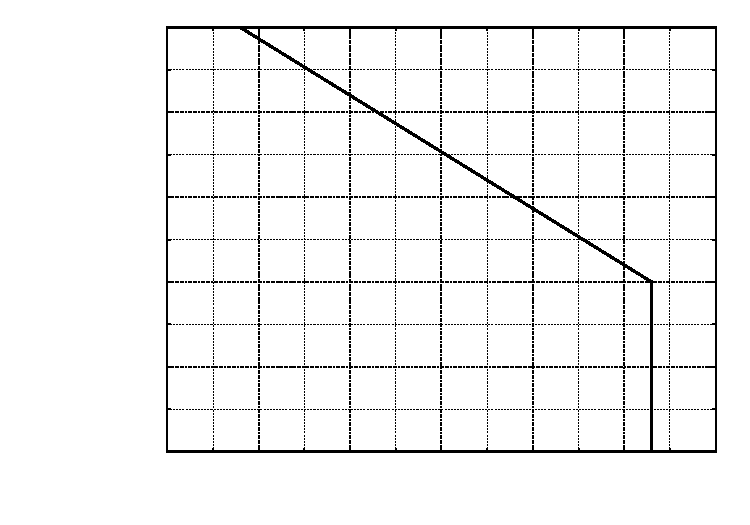
\includegraphics{../graphs/vne_chart}}%
    \gplfronttext
  \end{picture}%
\endgroup

  \end{center}  % chart from gnuplot
  \caption{$\mathrm{V_{NE}}$ vs Altitude}
  \end{figure}
\FloatBarrier

\section{AIRSPEED INDICATOR MARKINGS}

\begin{tabularx}{\textwidth}{|c|c|c|X|}
\hline 
MARKING&
ANALOG ASI&
EFIS&
SIGNIFICANCE\tabularnewline
&(KIAS)&(KIAS)&\tabularnewline

\hline
\hline 
White Arc&
48---87&
\textcolor{red}{48---87}&
Full Flap Operating Range. Lower limit is maximum weight stall speed
in landing configuration. Upper limit is maximum speed permissible
with flaps fully extended. \tabularnewline
\hline 
Green Arc&
50---168&
\textcolor{red}{50}---170&
Normal Operating Range. Lower limit is maximum weight stall speed
with flaps retracted. Upper limit is the maximum structural cruising
speed.\tabularnewline
\hline 
Yellow Arc&
168---200&
170---203&
Operations must be conducted with caution, and only in smooth air. \tabularnewline
\hline 
Red Line&
200&
203&
Maximum speed for all operations.\tabularnewline
\hline
\end{tabularx} 

\begin{Note}[NOTES]
\begin{enumerate}
\item The analog airspeed indicator markings are based on position
error estimates provided by Van's Aircraft. These markings do not account for the analog ASI instrument error (see Figure \ref{fg-asi-error}).

\item \textcolor{red}{The EFIS airspeed tape markings are to be revised
to incorporate actual position errors once these have been determined.}
\end{enumerate}
\end{Note}

\section{POWER PLANT LIMITATIONS}
The following limitations are for the Lycoming IO-360-A1B6
% No prop related RPM limits for this engine/prop combination.
\begin{longtable}[c]{@{}p{1.5in}p{4.25in}}
%\multicolumn{2}{@{}l}{Maximum Power\dotfill 200 hp}\\
\multicolumn{2}{@{}l}{Maximum Engine Speed\dotfill 2700 rpm}\\
Oil Temperature&Maximum\dotfill 245\textdegree F\\
&Desired\dotfill 180\textdegree F\\
&Minimum for continuous operation\dotfill 140\textdegree F\\
\\
\multicolumn{2}{@{}l}{Cylinder Head Temperature (CHT)}\\
&Maximum\dotfill 500\textdegree F\\
&75\% power cruise (Recommend max.)\dotfill 435\textdegree F\\
&Economy cruise  (Recommended maximum)\dotfill 400\textdegree F\\
&Recommended minimum for max. engine life\dotfill 150\textdegree F\\
\\
Oil pressure&Maximum (start, warm-up, taxi and takeoff)\dotfill115 psi\\
&Maximum (normal operations)\dotfill 95 psi\\
&Minimum (normal operations)\dotfill 55 psi\\
&Minimum (idle)\dotfill 25 psi\\
\\
Oil sump capacity&Maximum\dotfill8 US Qts\\
&Minimum safe quantity\dotfill 2 US Qts\\
\\
Fuel pressure&Maximum (at injector inlet)\dotfill 45 psi\\
&Minimum\dotfill 14 psi\\
\\
Fuel grade&Minimum Octane\dotfill 100/100LL Blue\\
\\
Propeller Diameter&Minimum\dotfill \textcolor{red}{72} inches\\
\end{longtable}


\section{ENGINE INSTRUMENT MARKINGS}
\begin{longtable}[c]{p{1.5in}p{4.25in}}
Tachometer&Green Arc --- Normal operating range. \dotfill 500 to 2700 rpm\\
&Red Line --- Maximum RPM\dotfill 2700 rpm\\
\end{longtable}

\section{EIS 4000 WARNING THRESHOLDS}
\begin{longtable}[c]{p{1.5in}p{4.25in}}
Oil Temperature&High Warning\dotfill 225\textdegree F\\
%&Low Warning \dotfill 140\textdegree F\\
\\
Oil Pressure&High Warning\dotfill 95 psi\\
% &Low Warning if rpm above \textcolor{red}{1500} rpm\dotfill 55 psi\\
% &Low Warning if rpm below \textcolor{red}{1500} rpm\dotfill 25 psi\\ 
&Low Warning\dotfill 25 psi\\ 
\\
Fuel Pressure&High Warning\dotfill 45 psi\\
&Low Warning\dotfill 14 psi\\
\\
CHT&High Warning\dotfill 450\textdegree F\\
%&Low Warning\dotfill 150\textdegree F\\
\\
RPM&High Warning\dotfill 2710 rpm\\
\\
Voltage&High Warning\dotfill 15 v\\
&Low Warning\dotfill 12 v\\
\\
Fuel Quantity&Low Level Warning\dotfill10 USG\\
\end{longtable}

\section{STARTER CRANKING LIMITATIONS}
The following limitations are for the SkyTec 149-12LS starter.
Starter cranking is limited to six 10 second cranking cycles with 20 second cool down between cranking attempts, then 30 minutes cooling.

\section{WEIGHT LIMITATIONS}
% if MTOW > 1800 lb, use this table (has line about MLW for non-paved strips)
\ifthenelse{\theMTOW > 1800}{
  \begin{longtable}[c]{p{1.5in}p{4.25in}}
    \multicolumn{2}{l}{Maximum Takeoff Weight\dotfill \theMTOW \space lb (\theMTOWkg .\theMTOWkgdecimal \space kg)}\\
    \multicolumn{2}{l}{Maximum Landing Weight\dotfill \theMTOW \space lb (\theMTOWkg .\theMTOWkgdecimal \space kg)}\\
    \multicolumn{2}{l}{Maximum weight for operations from non-paved runways\dotfill 1800 lb (816.5 kg)}\\
    \\
    \multicolumn{2}{l}{Aerobatic Gross weight (full 6g envelope available)\dotfill 1550 lb (703.1 kg)}\\
    \multicolumn{2}{l}{Restricted Aerobatic Gross weight (5g envelope available)\dotfill 1800 lb (816.5 kg)}\\
    \\
    \multicolumn{2}{l}{Maximum passenger weight\dotfill 300 lb (136 kg)}\\
    &\hfill (Subject to Weight \& Balance)\\
    \\
    \multicolumn{2}{l}{Maximum weight in forward baggage compartment\dotfill 50 lb (22.7 kg)}\\
    &\hfill (Subject to Weight \& Balance)\\
    \\
    \multicolumn{2}{l}{Maximum weight in rear baggage compartment\dotfill 75 lb (34 kg)}\\
    &\hfill (Subject to Weight \& Balance)\\
    \end{longtable}
  }
%if MTLOW <= 1800 lb, use the following table)
  {
    \begin{longtable}[c]{p{1.5in}p{4.25in}}
    \multicolumn{2}{l}{Maximum Takeoff Weight\dotfill \theMTOW \space lb (\theMTOWkg .\theMTOWkgdecimal \space kg)}\\
    \multicolumn{2}{l}{Maximum Landing Weight\dotfill \theMTOW \space lb (\theMTOWkg .\theMTOWkgdecimal \space kg)}\\
    \\
    \multicolumn{2}{l}{Aerobatic Gross weight (full 6g envelope available)\dotfill 1550 lb (703.1 kg)}\\
    \multicolumn{2}{l}{Restricted Aerobatic Gross weight (5g envelope available)\dotfill 1800 lb (816.5 kg)}\\
    \\
    \multicolumn{2}{l}{Maximum passenger weight\dotfill 300 lb (136 kg)}\\
    &\hfill (Subject to Weight \& Balance)\\
    \\
    \multicolumn{2}{l}{Maximum weight in forward baggage compartment\dotfill 50 lb (22.7 kg)}\\
    &\hfill (Subject to Weight \& Balance)\\
    \\
    \multicolumn{2}{l}{Maximum weight in rear baggage compartment\dotfill 75 lb (34 kg)}\\
    &\hfill (Subject to Weight \& Balance)\\
    \end{longtable}
  }

% only print the CAUTION if MTOW > 1800 lb
\ifthenelse{\theMTOW > 1800}
  {\begin{Note}[CAUTION]
  The maximum weight recommended by Van's Aircraft is 1800 lb  (816.5 kg).  Operations at higher weights must be conducted with caution.
  \end{Note}
   }
   {}


\begin{Note}[WARNING]
  The maximum weight recommended by Van's Aircraft for aerobatics is 1550 lb (703.1 kg).  Aerobatic operations at higher weights must respect reduced load factor limits.
  \end{Note}

\begin{Note}
  \textcolor{red}{The maximum passenger weight that is possible with the currently cleared aft CG of 85.3\char`\"{} aft of datum (aerobatic aft CG limit) is 250 lb  (113.4 kg).}
  \end{Note}



\section{CENTRE OF GRAVITY LIMITS}
\begin{longtable}[c]{p{1.5in}p{4.25in}}
\multicolumn{2}{l}{Forward limit\dotfill 15\% MAC = 78.7\char`\"{} aft of datum}\\
\multicolumn{2}{l}{Aft limit\dotfill 29\% MAC = 86.82\char`\"{} aft of datum}\\
\multicolumn{2}{l}{Aft limit for aerobatic flight\dotfill 26.5\% MAC = 85.3\char`\"{} aft of datum}\\
 & \\
\end{longtable}


\begin{Note}[NOTES]
\begin{enumerate*}
%\item The datum is 70\char`\"{} forward of the leading edge of the wing.\\
\item The datum is 70\char`\"{} forward of the leading edge of the wing.
\item  \textcolor{red}{The aft CG limit is currently restricted to  85.3\char`\"{} aft of datum (aerobatic aft CG limit) pending flight test validation of further aft CGs.}
\end{enumerate*}
\end{Note}

\begin{figure}[h!]
%\includegraphics*[viewport = 0 25 385 265]{../Diagrams/CG_envelope2.ps} % original chart from Grace
  \begin{center}
  \ifthenelse{\theMTOW > 1800}{% GNUPLOT: LaTeX picture with Postscript
\begingroup
  \makeatletter
  \providecommand\color[2][]{%
    \GenericError{(gnuplot) \space\space\space\@spaces}{%
      Package color not loaded in conjunction with
      terminal option `colourtext'%
    }{See the gnuplot documentation for explanation.%
    }{Either use 'blacktext' in gnuplot or load the package
      color.sty in LaTeX.}%
    \renewcommand\color[2][]{}%
  }%
  \providecommand\includegraphics[2][]{%
    \GenericError{(gnuplot) \space\space\space\@spaces}{%
      Package graphicx or graphics not loaded%
    }{See the gnuplot documentation for explanation.%
    }{The gnuplot epslatex terminal needs graphicx.sty or graphics.sty.}%
    \renewcommand\includegraphics[2][]{}%
  }%
  \providecommand\rotatebox[2]{#2}%
  \@ifundefined{ifGPcolor}{%
    \newif\ifGPcolor
    \GPcolorfalse
  }{}%
  \@ifundefined{ifGPblacktext}{%
    \newif\ifGPblacktext
    \GPblacktexttrue
  }{}%
  % define a \g@addto@macro without @ in the name:
  \let\gplgaddtomacro\g@addto@macro
  % define empty templates for all commands taking text:
  \gdef\gplbacktext{}%
  \gdef\gplfronttext{}%
  \makeatother
  \ifGPblacktext
    % no textcolor at all
    \def\colorrgb#1{}%
    \def\colorgray#1{}%
  \else
    % gray or color?
    \ifGPcolor
      \def\colorrgb#1{\color[rgb]{#1}}%
      \def\colorgray#1{\color[gray]{#1}}%
      \expandafter\def\csname LTw\endcsname{\color{white}}%
      \expandafter\def\csname LTb\endcsname{\color{black}}%
      \expandafter\def\csname LTa\endcsname{\color{black}}%
      \expandafter\def\csname LT0\endcsname{\color[rgb]{1,0,0}}%
      \expandafter\def\csname LT1\endcsname{\color[rgb]{0,1,0}}%
      \expandafter\def\csname LT2\endcsname{\color[rgb]{0,0,1}}%
      \expandafter\def\csname LT3\endcsname{\color[rgb]{1,0,1}}%
      \expandafter\def\csname LT4\endcsname{\color[rgb]{0,1,1}}%
      \expandafter\def\csname LT5\endcsname{\color[rgb]{1,1,0}}%
      \expandafter\def\csname LT6\endcsname{\color[rgb]{0,0,0}}%
      \expandafter\def\csname LT7\endcsname{\color[rgb]{1,0.3,0}}%
      \expandafter\def\csname LT8\endcsname{\color[rgb]{0.5,0.5,0.5}}%
    \else
      % gray
      \def\colorrgb#1{\color{black}}%
      \def\colorgray#1{\color[gray]{#1}}%
      \expandafter\def\csname LTw\endcsname{\color{white}}%
      \expandafter\def\csname LTb\endcsname{\color{black}}%
      \expandafter\def\csname LTa\endcsname{\color{black}}%
      \expandafter\def\csname LT0\endcsname{\color{black}}%
      \expandafter\def\csname LT1\endcsname{\color{black}}%
      \expandafter\def\csname LT2\endcsname{\color{black}}%
      \expandafter\def\csname LT3\endcsname{\color{black}}%
      \expandafter\def\csname LT4\endcsname{\color{black}}%
      \expandafter\def\csname LT5\endcsname{\color{black}}%
      \expandafter\def\csname LT6\endcsname{\color{black}}%
      \expandafter\def\csname LT7\endcsname{\color{black}}%
      \expandafter\def\csname LT8\endcsname{\color{black}}%
    \fi
  \fi
  \setlength{\unitlength}{0.0500bp}%
  \begin{picture}(7200.00,6300.00)%
    \gplgaddtomacro\gplbacktext{%
      \csname LTb\endcsname%
      \put(1210,704){\makebox(0,0)[r]{\strut{} 1100}}%
      \put(1210,1296){\makebox(0,0)[r]{\strut{} 1200}}%
      \put(1210,1889){\makebox(0,0)[r]{\strut{} 1300}}%
      \put(1210,2481){\makebox(0,0)[r]{\strut{} 1400}}%
      \put(1210,3073){\makebox(0,0)[r]{\strut{} 1500}}%
      \put(1210,3666){\makebox(0,0)[r]{\strut{} 1600}}%
      \put(1210,4258){\makebox(0,0)[r]{\strut{} 1700}}%
      \put(1210,4850){\makebox(0,0)[r]{\strut{} 1800}}%
      \put(1210,5443){\makebox(0,0)[r]{\strut{} 1900}}%
      \put(1210,6035){\makebox(0,0)[r]{\strut{} 2000}}%
      \put(1342,484){\makebox(0,0){\strut{} 78}}%
      \put(1895,484){\makebox(0,0){\strut{} 79}}%
      \put(2447,484){\makebox(0,0){\strut{} 80}}%
      \put(3000,484){\makebox(0,0){\strut{} 81}}%
      \put(3553,484){\makebox(0,0){\strut{} 82}}%
      \put(4106,484){\makebox(0,0){\strut{} 83}}%
      \put(4658,484){\makebox(0,0){\strut{} 84}}%
      \put(5211,484){\makebox(0,0){\strut{} 85}}%
      \put(5764,484){\makebox(0,0){\strut{} 86}}%
      \put(6316,484){\makebox(0,0){\strut{} 87}}%
      \put(6869,484){\makebox(0,0){\strut{} 88}}%
      \put(308,3369){\rotatebox{-270}{\makebox(0,0){\strut{}Weight (lb)}}}%
      \put(4105,154){\makebox(0,0){\strut{}CG (inches aft of datum)}}%
    }%
    \gplgaddtomacro\gplfronttext{%
      \put(3973,5147){\makebox(0,0){\strut{}Normal Weight/CG Envelope}}%
      \put(3553,4258){\makebox(0,0){\strut{}Restricted Aerobatic}}%
      \put(3553,3962){\makebox(0,0){\strut{}Weight/CG Envelope}}%
      \put(3553,2777){\makebox(0,0){\strut{}Aerobatic Weight/CG Envelope}}%
    }%
    \gplbacktext
    \put(0,0){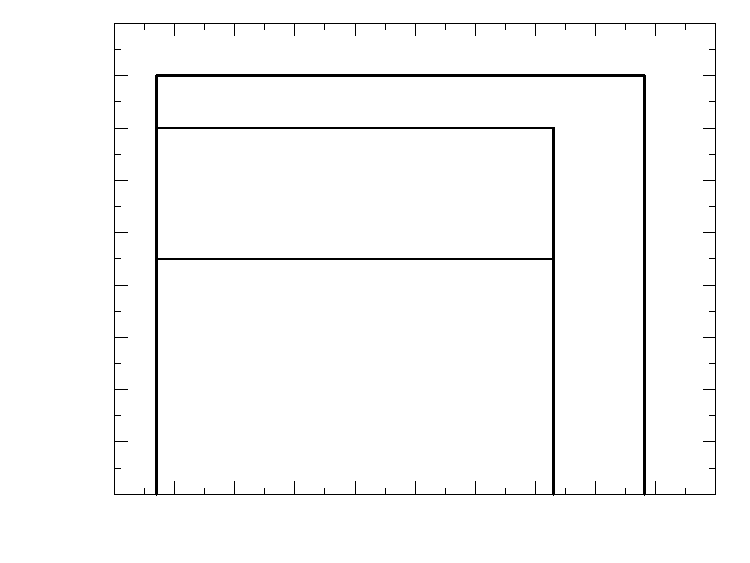
\includegraphics{../graphs/cg_chart1900}}%
    \gplfronttext
  \end{picture}%
\endgroup
}{% GNUPLOT: LaTeX picture with Postscript
\begingroup
  \makeatletter
  \providecommand\color[2][]{%
    \GenericError{(gnuplot) \space\space\space\@spaces}{%
      Package color not loaded in conjunction with
      terminal option `colourtext'%
    }{See the gnuplot documentation for explanation.%
    }{Either use 'blacktext' in gnuplot or load the package
      color.sty in LaTeX.}%
    \renewcommand\color[2][]{}%
  }%
  \providecommand\includegraphics[2][]{%
    \GenericError{(gnuplot) \space\space\space\@spaces}{%
      Package graphicx or graphics not loaded%
    }{See the gnuplot documentation for explanation.%
    }{The gnuplot epslatex terminal needs graphicx.sty or graphics.sty.}%
    \renewcommand\includegraphics[2][]{}%
  }%
  \providecommand\rotatebox[2]{#2}%
  \@ifundefined{ifGPcolor}{%
    \newif\ifGPcolor
    \GPcolorfalse
  }{}%
  \@ifundefined{ifGPblacktext}{%
    \newif\ifGPblacktext
    \GPblacktexttrue
  }{}%
  % define a \g@addto@macro without @ in the name:
  \let\gplgaddtomacro\g@addto@macro
  % define empty templates for all commands taking text:
  \gdef\gplbacktext{}%
  \gdef\gplfronttext{}%
  \makeatother
  \ifGPblacktext
    % no textcolor at all
    \def\colorrgb#1{}%
    \def\colorgray#1{}%
  \else
    % gray or color?
    \ifGPcolor
      \def\colorrgb#1{\color[rgb]{#1}}%
      \def\colorgray#1{\color[gray]{#1}}%
      \expandafter\def\csname LTw\endcsname{\color{white}}%
      \expandafter\def\csname LTb\endcsname{\color{black}}%
      \expandafter\def\csname LTa\endcsname{\color{black}}%
      \expandafter\def\csname LT0\endcsname{\color[rgb]{1,0,0}}%
      \expandafter\def\csname LT1\endcsname{\color[rgb]{0,1,0}}%
      \expandafter\def\csname LT2\endcsname{\color[rgb]{0,0,1}}%
      \expandafter\def\csname LT3\endcsname{\color[rgb]{1,0,1}}%
      \expandafter\def\csname LT4\endcsname{\color[rgb]{0,1,1}}%
      \expandafter\def\csname LT5\endcsname{\color[rgb]{1,1,0}}%
      \expandafter\def\csname LT6\endcsname{\color[rgb]{0,0,0}}%
      \expandafter\def\csname LT7\endcsname{\color[rgb]{1,0.3,0}}%
      \expandafter\def\csname LT8\endcsname{\color[rgb]{0.5,0.5,0.5}}%
    \else
      % gray
      \def\colorrgb#1{\color{black}}%
      \def\colorgray#1{\color[gray]{#1}}%
      \expandafter\def\csname LTw\endcsname{\color{white}}%
      \expandafter\def\csname LTb\endcsname{\color{black}}%
      \expandafter\def\csname LTa\endcsname{\color{black}}%
      \expandafter\def\csname LT0\endcsname{\color{black}}%
      \expandafter\def\csname LT1\endcsname{\color{black}}%
      \expandafter\def\csname LT2\endcsname{\color{black}}%
      \expandafter\def\csname LT3\endcsname{\color{black}}%
      \expandafter\def\csname LT4\endcsname{\color{black}}%
      \expandafter\def\csname LT5\endcsname{\color{black}}%
      \expandafter\def\csname LT6\endcsname{\color{black}}%
      \expandafter\def\csname LT7\endcsname{\color{black}}%
      \expandafter\def\csname LT8\endcsname{\color{black}}%
    \fi
  \fi
  \setlength{\unitlength}{0.0500bp}%
  \begin{picture}(7200.00,6300.00)%
    \gplgaddtomacro\gplbacktext{%
      \csname LTb\endcsname%
      \put(1210,704){\makebox(0,0)[r]{\strut{} 1100}}%
      \put(1210,1296){\makebox(0,0)[r]{\strut{} 1200}}%
      \put(1210,1889){\makebox(0,0)[r]{\strut{} 1300}}%
      \put(1210,2481){\makebox(0,0)[r]{\strut{} 1400}}%
      \put(1210,3073){\makebox(0,0)[r]{\strut{} 1500}}%
      \put(1210,3666){\makebox(0,0)[r]{\strut{} 1600}}%
      \put(1210,4258){\makebox(0,0)[r]{\strut{} 1700}}%
      \put(1210,4850){\makebox(0,0)[r]{\strut{} 1800}}%
      \put(1210,5443){\makebox(0,0)[r]{\strut{} 1900}}%
      \put(1210,6035){\makebox(0,0)[r]{\strut{} 2000}}%
      \put(1342,484){\makebox(0,0){\strut{} 78}}%
      \put(1895,484){\makebox(0,0){\strut{} 79}}%
      \put(2447,484){\makebox(0,0){\strut{} 80}}%
      \put(3000,484){\makebox(0,0){\strut{} 81}}%
      \put(3553,484){\makebox(0,0){\strut{} 82}}%
      \put(4106,484){\makebox(0,0){\strut{} 83}}%
      \put(4658,484){\makebox(0,0){\strut{} 84}}%
      \put(5211,484){\makebox(0,0){\strut{} 85}}%
      \put(5764,484){\makebox(0,0){\strut{} 86}}%
      \put(6316,484){\makebox(0,0){\strut{} 87}}%
      \put(6869,484){\makebox(0,0){\strut{} 88}}%
      \put(308,3369){\rotatebox{-270}{\makebox(0,0){\strut{}Weight (lb)}}}%
      \put(4105,154){\makebox(0,0){\strut{}CG (inches aft of datum)}}%
    }%
    \gplgaddtomacro\gplfronttext{%
      \put(5819,2777){\rotatebox{90}{\makebox(0,0){\strut{}Normal Weight/CG Envelope}}}%
      \put(3553,4258){\makebox(0,0){\strut{}Restricted Aerobatic}}%
      \put(3553,3962){\makebox(0,0){\strut{}Weight/CG Envelope}}%
      \put(3553,2777){\makebox(0,0){\strut{}Aerobatic Weight/CG Envelope}}%
    }%
    \gplbacktext
    \put(0,0){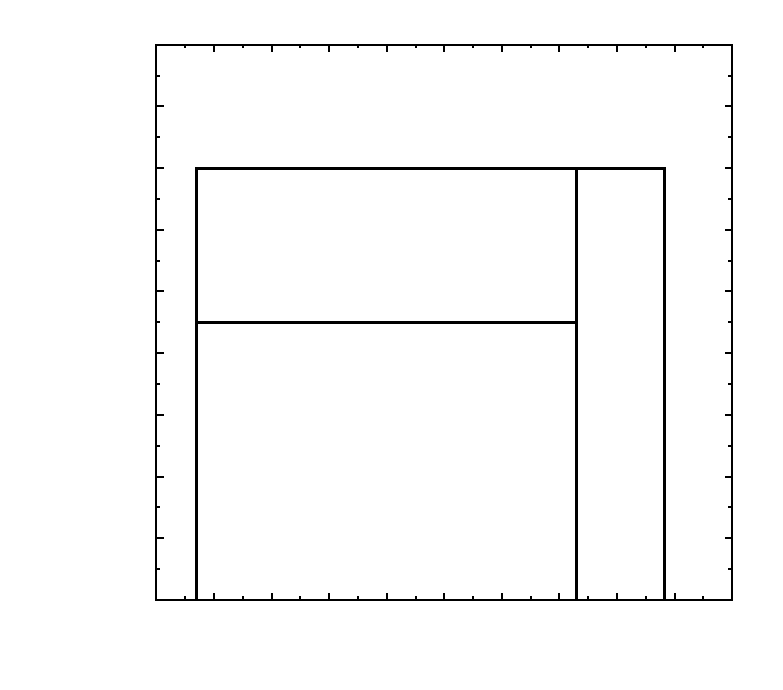
\includegraphics{../graphs/cg_chart1800}}%
    \gplfronttext
  \end{picture}%
\endgroup
}
  \end{center}  % chart from gnuplot
  \caption{Centre of Gravity Limits}
  \end{figure}
\FloatBarrier
%\pagebreak[4]
\section{MANOEUVRE LIMITS}
The following list of manoeuvres is approved when operating within the Restricted Aerobatic Weight/CG Envelope.

\begin{itemize*}
\item Upright spins, 
\item Loops, 
\item Cuban Eights, 
\item Immelmann turns, 
\item Aileron Rolls, and
\item Barrel rolls.
\end{itemize*}




% The following additional manoeuvres are approved when operating within the Aerobatic Weight/CG Envelope.

%\begin{itemize*}
%\item Hammerhead stalls, 
%\item Snap Rolls (maximum allowable entry speed
%is 95 KIAS), \item Vertical rolls, and \item Split-S (maximum allowable entry
%speed is 95 KIAS).
%\end{itemize*}
%

% \addpenalty used to suggest this is a good place to possibly break a page.
%\addpenalty{-750}
\section{LOAD FACTOR LIMITS}
\newlength{\loadcolonewidth}
\setlength{\loadcolonewidth}{0.25in}

\begin{tabular}[c]{p{.25in}p{5.5in}}
  \multicolumn{2}{l}{Load Factor Limits}\\ 
 &Flaps Up\\
  &\hspace*{\loadcolonewidth}weight 1550 lb (703.1 kg) and below:\dotfill +6g to -3g\\
  &\hspace*{\loadcolonewidth}reducing linearly to - weight  1800 lb (816.5 kg):\dotfill +5g to -2.5g\\
%  &\hspace*{\loadcolonewidth}weight 1800 lb (816.5 kg)\dotfill +5g to -2.5g\\
  \ifthenelse{\theMTOW > 1800}{
  &\hspace*{\loadcolonewidth}weight above 1800 lb (816.5 kg):\dotfill +4.4g to -2g\-\\\\
  }
  {}
  &Flaps Down\dotfill +2g to 0g\\
  \end{tabular}


\begin{NoteCtr}
  The load factor limit varies linearly between 1800 lb  (816.5 kg) and 1550 lb (703.1 kg) weight.
  \end{NoteCtr}

\begin{NoteCtr}[Caution]
  While the airframe is stressed for negative g, the engine does not have an inverted oil system.
  \end{NoteCtr}

\begin{figure}[htb]
  \begin{center}
  \ifthenelse{\theMTOW > 1800}{% GNUPLOT: LaTeX picture with Postscript
\begingroup
  \makeatletter
  \providecommand\color[2][]{%
    \GenericError{(gnuplot) \space\space\space\@spaces}{%
      Package color not loaded in conjunction with
      terminal option `colourtext'%
    }{See the gnuplot documentation for explanation.%
    }{Either use 'blacktext' in gnuplot or load the package
      color.sty in LaTeX.}%
    \renewcommand\color[2][]{}%
  }%
  \providecommand\includegraphics[2][]{%
    \GenericError{(gnuplot) \space\space\space\@spaces}{%
      Package graphicx or graphics not loaded%
    }{See the gnuplot documentation for explanation.%
    }{The gnuplot epslatex terminal needs graphicx.sty or graphics.sty.}%
    \renewcommand\includegraphics[2][]{}%
  }%
  \providecommand\rotatebox[2]{#2}%
  \@ifundefined{ifGPcolor}{%
    \newif\ifGPcolor
    \GPcolorfalse
  }{}%
  \@ifundefined{ifGPblacktext}{%
    \newif\ifGPblacktext
    \GPblacktexttrue
  }{}%
  % define a \g@addto@macro without @ in the name:
  \let\gplgaddtomacro\g@addto@macro
  % define empty templates for all commands taking text:
  \gdef\gplbacktext{}%
  \gdef\gplfronttext{}%
  \makeatother
  \ifGPblacktext
    % no textcolor at all
    \def\colorrgb#1{}%
    \def\colorgray#1{}%
  \else
    % gray or color?
    \ifGPcolor
      \def\colorrgb#1{\color[rgb]{#1}}%
      \def\colorgray#1{\color[gray]{#1}}%
      \expandafter\def\csname LTw\endcsname{\color{white}}%
      \expandafter\def\csname LTb\endcsname{\color{black}}%
      \expandafter\def\csname LTa\endcsname{\color{black}}%
      \expandafter\def\csname LT0\endcsname{\color[rgb]{1,0,0}}%
      \expandafter\def\csname LT1\endcsname{\color[rgb]{0,1,0}}%
      \expandafter\def\csname LT2\endcsname{\color[rgb]{0,0,1}}%
      \expandafter\def\csname LT3\endcsname{\color[rgb]{1,0,1}}%
      \expandafter\def\csname LT4\endcsname{\color[rgb]{0,1,1}}%
      \expandafter\def\csname LT5\endcsname{\color[rgb]{1,1,0}}%
      \expandafter\def\csname LT6\endcsname{\color[rgb]{0,0,0}}%
      \expandafter\def\csname LT7\endcsname{\color[rgb]{1,0.3,0}}%
      \expandafter\def\csname LT8\endcsname{\color[rgb]{0.5,0.5,0.5}}%
    \else
      % gray
      \def\colorrgb#1{\color{black}}%
      \def\colorgray#1{\color[gray]{#1}}%
      \expandafter\def\csname LTw\endcsname{\color{white}}%
      \expandafter\def\csname LTb\endcsname{\color{black}}%
      \expandafter\def\csname LTa\endcsname{\color{black}}%
      \expandafter\def\csname LT0\endcsname{\color{black}}%
      \expandafter\def\csname LT1\endcsname{\color{black}}%
      \expandafter\def\csname LT2\endcsname{\color{black}}%
      \expandafter\def\csname LT3\endcsname{\color{black}}%
      \expandafter\def\csname LT4\endcsname{\color{black}}%
      \expandafter\def\csname LT5\endcsname{\color{black}}%
      \expandafter\def\csname LT6\endcsname{\color{black}}%
      \expandafter\def\csname LT7\endcsname{\color{black}}%
      \expandafter\def\csname LT8\endcsname{\color{black}}%
    \fi
  \fi
  \setlength{\unitlength}{0.0500bp}%
  \begin{picture}(7200.00,5040.00)%
    \gplgaddtomacro\gplbacktext{%
      \csname LTb\endcsname%
      \put(814,704){\makebox(0,0)[r]{\strut{}-4}}%
      \csname LTb\endcsname%
      \put(814,1444){\makebox(0,0)[r]{\strut{}-2}}%
      \csname LTb\endcsname%
      \put(814,2184){\makebox(0,0)[r]{\strut{} 0}}%
      \csname LTb\endcsname%
      \put(814,2925){\makebox(0,0)[r]{\strut{} 2}}%
      \csname LTb\endcsname%
      \put(814,3665){\makebox(0,0)[r]{\strut{} 4}}%
      \csname LTb\endcsname%
      \put(814,4405){\makebox(0,0)[r]{\strut{} 6}}%
      \csname LTb\endcsname%
      \put(946,484){\makebox(0,0){\strut{} 1100}}%
      \csname LTb\endcsname%
      \put(1604,484){\makebox(0,0){\strut{} 1200}}%
      \csname LTb\endcsname%
      \put(2262,484){\makebox(0,0){\strut{} 1300}}%
      \csname LTb\endcsname%
      \put(2920,484){\makebox(0,0){\strut{} 1400}}%
      \csname LTb\endcsname%
      \put(3578,484){\makebox(0,0){\strut{} 1500}}%
      \csname LTb\endcsname%
      \put(4237,484){\makebox(0,0){\strut{} 1600}}%
      \csname LTb\endcsname%
      \put(4895,484){\makebox(0,0){\strut{} 1700}}%
      \csname LTb\endcsname%
      \put(5553,484){\makebox(0,0){\strut{} 1800}}%
      \csname LTb\endcsname%
      \put(6211,484){\makebox(0,0){\strut{} 1900}}%
      \csname LTb\endcsname%
      \put(6869,484){\makebox(0,0){\strut{} 2000}}%
      \put(308,2739){\rotatebox{-270}{\makebox(0,0){\strut{}Load Factor Limit (g)}}}%
      \put(3907,154){\makebox(0,0){\strut{}Weight (lb)}}%
    }%
    \gplgaddtomacro\gplfronttext{%
    }%
    \gplbacktext
    \put(0,0){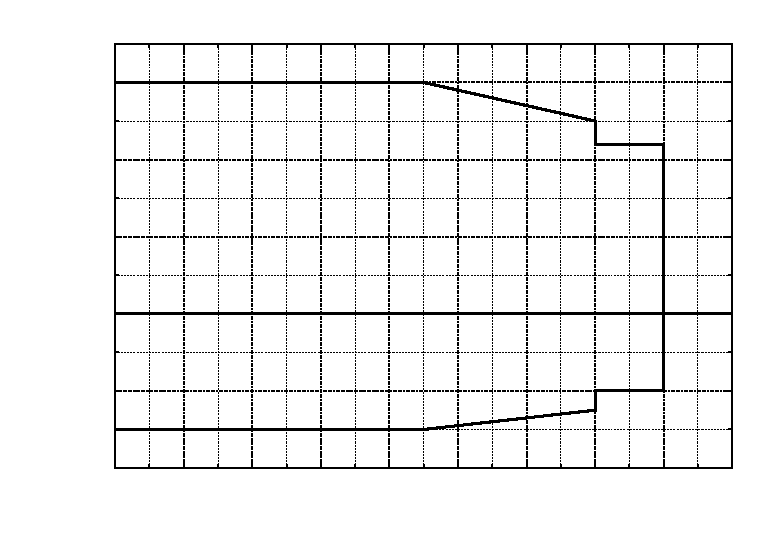
\includegraphics{../graphs/g-chart1900}}%
    \gplfronttext
  \end{picture}%
\endgroup
}{% GNUPLOT: LaTeX picture with Postscript
\begingroup
  \makeatletter
  \providecommand\color[2][]{%
    \GenericError{(gnuplot) \space\space\space\@spaces}{%
      Package color not loaded in conjunction with
      terminal option `colourtext'%
    }{See the gnuplot documentation for explanation.%
    }{Either use 'blacktext' in gnuplot or load the package
      color.sty in LaTeX.}%
    \renewcommand\color[2][]{}%
  }%
  \providecommand\includegraphics[2][]{%
    \GenericError{(gnuplot) \space\space\space\@spaces}{%
      Package graphicx or graphics not loaded%
    }{See the gnuplot documentation for explanation.%
    }{The gnuplot epslatex terminal needs graphicx.sty or graphics.sty.}%
    \renewcommand\includegraphics[2][]{}%
  }%
  \providecommand\rotatebox[2]{#2}%
  \@ifundefined{ifGPcolor}{%
    \newif\ifGPcolor
    \GPcolorfalse
  }{}%
  \@ifundefined{ifGPblacktext}{%
    \newif\ifGPblacktext
    \GPblacktexttrue
  }{}%
  % define a \g@addto@macro without @ in the name:
  \let\gplgaddtomacro\g@addto@macro
  % define empty templates for all commands taking text:
  \gdef\gplbacktext{}%
  \gdef\gplfronttext{}%
  \makeatother
  \ifGPblacktext
    % no textcolor at all
    \def\colorrgb#1{}%
    \def\colorgray#1{}%
  \else
    % gray or color?
    \ifGPcolor
      \def\colorrgb#1{\color[rgb]{#1}}%
      \def\colorgray#1{\color[gray]{#1}}%
      \expandafter\def\csname LTw\endcsname{\color{white}}%
      \expandafter\def\csname LTb\endcsname{\color{black}}%
      \expandafter\def\csname LTa\endcsname{\color{black}}%
      \expandafter\def\csname LT0\endcsname{\color[rgb]{1,0,0}}%
      \expandafter\def\csname LT1\endcsname{\color[rgb]{0,1,0}}%
      \expandafter\def\csname LT2\endcsname{\color[rgb]{0,0,1}}%
      \expandafter\def\csname LT3\endcsname{\color[rgb]{1,0,1}}%
      \expandafter\def\csname LT4\endcsname{\color[rgb]{0,1,1}}%
      \expandafter\def\csname LT5\endcsname{\color[rgb]{1,1,0}}%
      \expandafter\def\csname LT6\endcsname{\color[rgb]{0,0,0}}%
      \expandafter\def\csname LT7\endcsname{\color[rgb]{1,0.3,0}}%
      \expandafter\def\csname LT8\endcsname{\color[rgb]{0.5,0.5,0.5}}%
    \else
      % gray
      \def\colorrgb#1{\color{black}}%
      \def\colorgray#1{\color[gray]{#1}}%
      \expandafter\def\csname LTw\endcsname{\color{white}}%
      \expandafter\def\csname LTb\endcsname{\color{black}}%
      \expandafter\def\csname LTa\endcsname{\color{black}}%
      \expandafter\def\csname LT0\endcsname{\color{black}}%
      \expandafter\def\csname LT1\endcsname{\color{black}}%
      \expandafter\def\csname LT2\endcsname{\color{black}}%
      \expandafter\def\csname LT3\endcsname{\color{black}}%
      \expandafter\def\csname LT4\endcsname{\color{black}}%
      \expandafter\def\csname LT5\endcsname{\color{black}}%
      \expandafter\def\csname LT6\endcsname{\color{black}}%
      \expandafter\def\csname LT7\endcsname{\color{black}}%
      \expandafter\def\csname LT8\endcsname{\color{black}}%
    \fi
  \fi
  \setlength{\unitlength}{0.0500bp}%
  \begin{picture}(7200.00,5040.00)%
    \gplgaddtomacro\gplbacktext{%
      \csname LTb\endcsname%
      \put(814,704){\makebox(0,0)[r]{\strut{}-4}}%
      \csname LTb\endcsname%
      \put(814,1444){\makebox(0,0)[r]{\strut{}-2}}%
      \csname LTb\endcsname%
      \put(814,2184){\makebox(0,0)[r]{\strut{} 0}}%
      \csname LTb\endcsname%
      \put(814,2925){\makebox(0,0)[r]{\strut{} 2}}%
      \csname LTb\endcsname%
      \put(814,3665){\makebox(0,0)[r]{\strut{} 4}}%
      \csname LTb\endcsname%
      \put(814,4405){\makebox(0,0)[r]{\strut{} 6}}%
      \csname LTb\endcsname%
      \put(946,484){\makebox(0,0){\strut{} 1100}}%
      \csname LTb\endcsname%
      \put(1604,484){\makebox(0,0){\strut{} 1200}}%
      \csname LTb\endcsname%
      \put(2262,484){\makebox(0,0){\strut{} 1300}}%
      \csname LTb\endcsname%
      \put(2920,484){\makebox(0,0){\strut{} 1400}}%
      \csname LTb\endcsname%
      \put(3578,484){\makebox(0,0){\strut{} 1500}}%
      \csname LTb\endcsname%
      \put(4237,484){\makebox(0,0){\strut{} 1600}}%
      \csname LTb\endcsname%
      \put(4895,484){\makebox(0,0){\strut{} 1700}}%
      \csname LTb\endcsname%
      \put(5553,484){\makebox(0,0){\strut{} 1800}}%
      \csname LTb\endcsname%
      \put(6211,484){\makebox(0,0){\strut{} 1900}}%
      \csname LTb\endcsname%
      \put(6869,484){\makebox(0,0){\strut{} 2000}}%
      \put(308,2739){\rotatebox{-270}{\makebox(0,0){\strut{}Load Factor Limit (g)}}}%
      \put(3907,154){\makebox(0,0){\strut{}Weight (lb)}}%
    }%
    \gplgaddtomacro\gplfronttext{%
    }%
    \gplbacktext
    \put(0,0){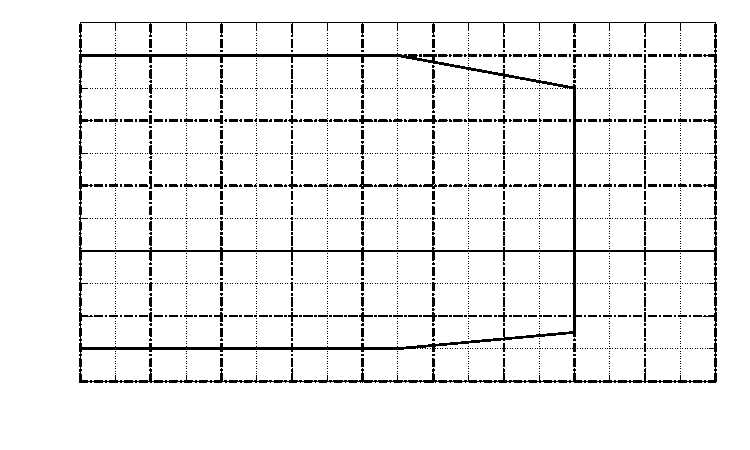
\includegraphics{../graphs/g-chart1800}}%
    \gplfronttext
  \end{picture}%
\endgroup
}
  \end{center}  % chart from gnuplot
  \caption{Load Factor Limit vs Weight}
  \end{figure}
  
\begin{Note}[NOTES]
  \begin{enumerate}
    \item The load factor limits for weights above 1550 lb (703.1 kg) are not published by
Van's Aircraft, but are established based on conservative engineering
analysis of wing bending moment vs load factor. 
    \item The load factor limits for flaps down are based on FAR
23 structural design criteria, which the RV-8 is designed to.  
    \end{enumerate}
  \end{Note}

\section{KINDS OF OPERATION LIMITS}

The airplane is approved for:
\begin{itemize*}
\item Day VFR,
\item Night VFR (\textcolor{red}{subject to flight test validation of night lighting}), 
\item Day IFR, and 
\item Night IFR (\textcolor{red}{subject to flight test validation of night lighting}).
\end{itemize*}
Flight in known or forecast icing conditions is prohibited.


\section{FUEL LIMITATIONS}
\begin{quote}
Total capacity\dotfill 163.5 l (43.2 USG)\\
Usable fuel\dotfill 43 USG\\
Unusable fuel\dotfill 0.2 USG\\
Approved fuels\dotfill 100/130 - Green\\
%\raggedleft 100 - Green\\
%100LL - Blue\\
\hspace*{\fill}100 - Green\\
\hspace*{\fill}100LL - Blue\\
\end{quote}

It is prohibited to select the left tank for takeoff or landing
unless there are at least \textcolor{red}{10 USG} of fuel remaining in the selected tank.  

%\section{ELECTRICAL LIMITATIONS}
%Aux Power -- The Aux Power receptacle is limited to 10 amps maximum.

\section{GNS 430W LIMITATIONS}
%
%  The Main software version is displayed on the GNS 430W self test page immediately after turn-on for 5 seconds.  The remaining system software versions can be verified on the AUX group sub-page 2, "SOFTWARE/DATABASE VER".


  IFR enroute and terminal navigation predicated upon the GNS 430W's GPS receiver is prohibited unless the pilot verifies the currency of the data base or verifies each selected waypoint for accuracy by reference to current approved data.
  
  Operations on RNAV STARs are prohibited unless the autopilot is engaged in TRK mode (TC AIM RAC 9.2.2 \& FAA AC 90-100A para 10(b)(9)).
  
  Instrument approach navigation predicated upon the GNS 430W's GPS receiver must be accomplished in accordance with approved instrument approach procedures that are retrieved from the GNS 430W's data base.  The GNS 430W's database must incorporate the current update cycle.
  \begin{enumerate}
    \item Instrument approaches utilizing the GPS receiver must be conducted in the Approach Mode and Receiver Autonomous Integrity Monitoring (RAIM) must be available at the Final Approach Fix.
    \item Accomplishment of ILS, LOC, LOC-BC, LDA, SDF, MLS or any other type of approach not approved for GPS overlay with the GNS 430W's GPS receiver is not authorized.
    \item Use of the GNS 430W's VOR/ILS receiver to fly approaches not approved for GPS require VOR/ILS navigation data to be displayed on the external indicator.
    \item VNAV information may be utilized for advisory information only. Use of VNAV information for instrument approach procedures does not guarantee step-down fix altitude protection, or arrival at approach minimums in normal position to land.
    \end{enumerate}
  If not previously defined, the following default settings must be made in the ``SETUP 1'' menu of the GNS 430W prior to operation (refer to GNS 430W Pilot's Guide for procedure if necessary):

  \begin{tabular}{ll}
     \textbf{dis, spd} &nm, kt (sets navigation units to ``nautical miles'' and ``knots'')\\
     \textbf{alt, vs} &ft, fpm (sets altitude units to ``feet'' and ``feet per minute'')\\
     \textbf{map datum} &WGS 84 (sets map datum to WGS-84)\\
     \textbf{posn} &deg-min (sets navigation grid units to decimal minutes)\\
     \end{tabular}

\section{AUTOPILOT LIMITATIONS}
Minimum engage height: 400 ft AGL.

%Preflight override test must be conducted if wing leveler is to be used on that flight.
Use of the autopilot in-flight is prohibited unless pre-flight override tests were conducted on both pitch and roll axis.
%\textcolor{red}{add more if required}
\clearpage
\section{PLACARDS}
The following information is displayed by placards:

\settowidth{\colOne}{Forward Baggage Area}
%\setlength{\colTwo}{\textwidth-\colOne-24pt}
%%\setlength{\colTwo}{4in}

\begin{tabularx}{\textwidth}{p{\colOne}X}
  \textbf{Location}&\textbf{Placard}\\
  Front Seat&THE FOLLOWING  AEROBATIC MANOEUVRES, AND COMBINATIONS THEREOF, MAY BE PERFORMED IN THIS AEROPLANE:\\
 % \textcolor{red}{(List approved manoeuvres, once they are defined - see AMA 549.101A \S5a.)}\\
&\begin{itemize*}
\item UPRIGHT SPINS, 
\item LOOPS, 
\item CUBAN EIGHTS, 
\item IMMELMANN TURNS, 
\item AILERON ROLLS, AND
\item BARREL ROLLS.
\end{itemize*}\\
  \raggedright Ahead of Throttle Quadrant&
  \begin{tabular}{ccccc}
    \multicolumn{5}{c}{MAXIMUM POWER MIXTURE}\\
    ALTITUDE&S.L.&4000&8000&12,000\\
    US GAL/HR&17&15&13&10\\
    \end{tabular}\\\\
  \raggedright Rear Seat& YOU FLY IN THIS AIRCRAFT AT YOUR OWN RISK.  THIS AIRCRAFT DOES NOT COMPLY WITH INTERNATIONALLY RECOGNIZED STANDARDS. VOUS VOLEZ \`{A} BORD DE CET A\'{E}RONEF  \`{A} VOS PROPRES RISQUES.  CET A\'{E}RONEF N�EST PAS CONFORME AUX NORMES RECONNUES  \`{A} L�\'{E}CHELLE INTERNATIONALE.\\\\
  % Rear Seat& PASSENGERS PROHIBITED \textcolor{red}{(Placard only required during Flight Test Phase)} \\\\
  Rear Seat&MAXIMUM  PASSENGER LOAD 136 KG (300  LB)\\\\
  Forward Baggage Area&MAXIMUM BAGGAGE LOAD 23 KG (50 LB)\\\\
  Aft Baggage Area&MAXIMUM BAGGAGE LOAD 34 KG (75 LB)\\\\
  % By Fuel Tank Cap&FUEL CAPACITY \textcolor{red}{159} L 100 LL OR 100/130 \textcolor{red}{(Check required wording.)}
  \end{tabularx}

\cleardoublepage
